\documentclass{article}

\usepackage{amsmath}
\usepackage{amssymb}
\usepackage{parskip}
\usepackage{fullpage}
\usepackage{hyperref}
\usepackage{pgfplots}
\usepackage{wrapfig}
\usetikzlibrary{calc}

\hypersetup{
    colorlinks=true,
    linkcolor=black,
    urlcolor=blue,
    pdftitle={DifferentialEquations},
    pdfpagemode=FullScreen,
}

\title{Differential Equations}
\author{Paolo Bettelini}
\date{}

\begin{document}

\maketitle
\tableofcontents
\pagebreak

\section{Definition}

Differential equations are equations where the solution is a function
or a set of functions.

\section{Slope Field}

A slope field or directional field is a field to visualize
solutions to a first-order differential equation.

\begin{wrapfigure}[15]{l}{7.5cm} % 10 is the number of wrapfigure lines
    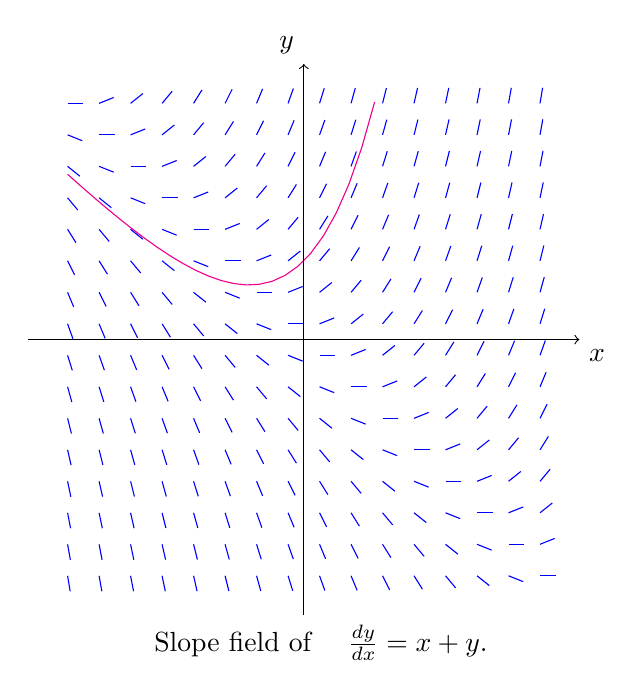
\begin{tikzpicture}[declare function={f(\x,\y)=\x+\y;}]
        \def\xmax{3} \def\xmin{-3}
        \def\ymax{3} \def\ymin{-3}
        \def\nx{15}
        \def\ny{15}
        
        \pgfmathsetmacro{\hx}{(\xmax-\xmin)/\nx}
        \pgfmathsetmacro{\hy}{(\ymax-\ymin)/\ny}
        \foreach \i in {0,...,\nx}
            \foreach \j in {0,...,\ny}{
                \pgfmathsetmacro{\yprime}{f({\xmin+\i*\hx},{\ymin+\j*\hy})}
                \draw[blue,shift={({\xmin+\i*\hx},{\ymin+\j*\hy})}] 
                (0,0)--($(0,0)!2mm!(.1,.1*\yprime)$);
            }
        
        % a solution y=(yo+1)e^x-x-1
        \def\yo{1}
        \draw[magenta] plot[domain=\xmin:.9] (\x,{(\yo+1)*exp(\x)-\x-1});
        
        \draw[->] (\xmin-.5,0)--(\xmax+.5,0) node[below right] {\(x\)};
        \draw[->] (0,\ymin-.5)--(0,\ymax+.5) node[above left] {\(y\)};
        
        \draw (current bounding box.south) node[below]
        {Slope field of \quad \(\frac{dy}{dx}=x+y\).};
    \end{tikzpicture}

\end{wrapfigure}

\phantom{ } \\

This field is obtained by picking points on the plane. \\
For each point \((x,y)\) we know that the slope \((\frac{dy}{dx})\)
is \(x + y\). \\
This means that if a solution passes through \((x,y)\), then its slope is \(x+y\). \\
The red curve shows a solution.

% this is embarassing
% I don't know how to deal with wrapfig
\phantom{ } \\
\phantom{ } \\
\phantom{ } \\
\phantom{ } \\
\phantom{ } \\
\phantom{ } \\
\phantom{ } \\
\phantom{ } \\
\phantom{ } \\
\phantom{ } \\
\phantom{ } \\

\section{Euler's Method}

Euler's method is a technique for solving a 
first-order differential equation numerically given a point of the solution.
\\
Starting at the known solution point \(A_0\), we take small steps the direction
of the slope field. As the length of the steps \(s \to 0\)
we approach the solution to the equation. \\
The angle of the slope is given by
\[
    \theta = \tan\left(\frac{dy}{dx}\right)
    \]
so each step gives the sequence of points
\[
    A_n = A_{n_1} \cdot s \left(\cos(\theta), \sin(\theta)\right)
\]

\pagebreak

\end{document}
